\chapter{创新点1}
	\label{chapter_novel_idea_1}
	这里是创新点1。
	\begin{figure}[htb]
		\centering 
			\subfigure[]{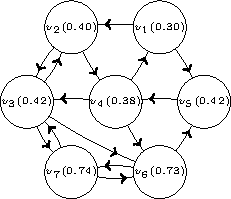
\includegraphics[scale=1]{fig/novel_idea_1/NG1.pdf}}
			\subfigure[]{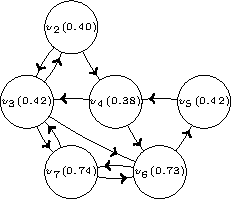
\includegraphics[scale=1]{fig/novel_idea_1/NG2.pdf}}
			\subfigure[]{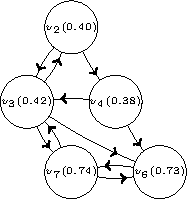
\includegraphics[scale=1]{fig/novel_idea_1/NG3.pdf}}
			\subfigure[]{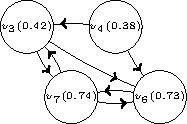
\includegraphics[scale=1]{fig/novel_idea_1/NG4.pdf}}
			\subfigure[]{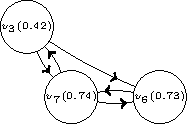
\includegraphics[scale=1]{fig/novel_idea_1/NG5.pdf}}
			\subfigure[]{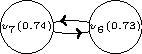
\includegraphics[scale=1]{fig/novel_idea_1/NG6.pdf}}
			\subfigure[]{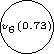
\includegraphics[scale=1]{fig/novel_idea_1/NG7.pdf}}
		\caption{NearestGraph算法实例转化图}
		\label{fig_QoS_distribution}
	\end{figure} 

	\begin{table}[htb]
		\caption{QoS数据集的数字特征}
		\label{table_Dataset_Statics}
		\centering
		\scalebox{0.85}[0.85]{
		\begin{tabular}{lll}
		\toprule  %添加表格头部粗线
		Statics &\quad Response-Time(seconds) &\quad Throughput(kbps)\\
		\hline
		Value Range &\qquad(0,20) &\qquad(0,1000)\\
		Mean &\qquad 0.910 &\qquad 47.386\\
		Median &\qquad 0.3320 &\qquad 11.07\\
		Standard Variance &\qquad 1.9320 &\qquad 107.4093\\
		User Num &\qquad 339 &\qquad 339\\
		Service Num &\qquad 5828 &\qquad 5828\\
		Records Num &\qquad 1974675 &\qquad 1974675\\
		\bottomrule %添加表格底部粗线
		\end{tabular}}
	\end{table}

	\begin{table}[htb]
		\centering
		\caption{性能对比}
		\label{table_Performance_Comparisons}
		\scalebox{0.7}[0.7]{
		\begin{tabular}{llllllll}
		\toprule
		Matrix &\multirow{2}*{Metrics\quad}&\multicolumn{6}{c}{Response-Time(seconds)}\\
		\cline{3-8}
		Density(\%)\qquad\quad& & UMean\qquad\qquad& IMean\qquad\qquad& UPCC\qquad\qquad& IPCC\qquad\qquad& WSRec\qquad\qquad& NearestGraph\\
		\multirow{2}*{10}& MAE& 0.8785& 0.7015& 0.6761& 0.6897& 0.6679& \textbf{0.6643}\\
		& RMSE& 1.8591& 1.5813& 1.4078& 1.4296& 1.4053& \textbf{1.4027}\\
		\multirow{2}*{20}& MAE& 0.8768& 0.6867& 0.5517& 0.5917& 0.5431& \textbf{0.5104}\\
		& RMSE& 1.8548& 1.5342& 1.3151& 1.3268& 1.2986& \textbf{1.2785}\\	
		\multirow{2}*{30}& MAE& 0.8747& 0.6818& 0.5159& 0.5037& 0.4927& \textbf{0.4723}\\
		& RMSE& 1.8557& 1.5311& 1.2680& 1.2252& 1.1973& \textbf{1.1246}\\
		\toprule
		Matrix&\multirow{2}*{Metrics\quad}&\multicolumn{6}{c}{Throughput(kbps)}\\
		\cline{3-8}
		Density(\%)\qquad\quad& & UMean\qquad\qquad& IMean\qquad\qquad& UPCC\qquad\qquad& IPCC\qquad\qquad& WSRec\qquad\qquad& NearestGraph\\
		\multirow{2}*{10}& MAE& 54.0084& 29.2651& 26.1230& 29.2651& 24.3285& \textbf{24.3269}\\
		& RMSE& 110.2821& 66.6334& 63.9573& 64.2285& 64.1908& \textbf{63.5435}\\
		\multirow{2}*{20}& MAE& 53.6768& 27.3393& 24.2695& 26.8318& 22.7717& \textbf{21.7493}\\
		& RMSE& 110.2977& 64.3986& 54.4783& 60.0825& 54.3701& \textbf{52.8731}\\	
		\multirow{2}*{30}& MAE& 53.8792& 26.6239& 23.7455& 26.4319& 21.3194& \textbf{19.6530}\\
		& RMSE& 110.1751& 64.3986& 54.4783& 57.8593& 51.7768& \textbf{50.5765}\\
		\bottomrule	
		\end{tabular}}
		\end{table}